% option draft um zu lange Zeilen anzuzeigen
\documentclass[a4paper,11pt,draft]{article}

\usepackage[inner=3cm,outer=3cm]{geometry}
\usepackage[english]{babel}
\usepackage[utf8]{inputenc}
% linux libertine for normal text
\usepackage{libertine}
\usepackage{libertinust1math}
% inconsolate as teletype font
\usepackage{inconsolata}
\usepackage[T1]{fontenc}
\usepackage{color}
\usepackage{graphicx}
\usepackage{wrapfig}
\usepackage{amsmath}
\usepackage{amssymb}
\usepackage{mathastext}
\usepackage{subcaption}
\usepackage{pmboxdraw}
\usepackage{lipsum}
\usepackage[export]{adjustbox}
\usepackage{csquotes}
\usepackage{tabularx}
\usepackage[sort]{natbib}
\usepackage[toc,nonumberlist]{glossaries}
\usepackage{makecell}
\usepackage[absolute,overlay]{textpos}
\usepackage{microtype}
\usepackage[linesnumbered,ruled]{algorithm2e}

% setup of siunitx
\usepackage[binary-units=true]{siunitx}
\DeclareSIUnit{\bits}{bits}
\DeclareSIUnit{\cycle}{cycle}
\DeclareSIUnit{\cycles}{cycles}
\sisetup{
  list-final-separator = {, and },
  per-mode=symbol
}

% tikz
\usepackage{tikz}
\usepackage{tikz-uml}
\usetikzlibrary{arrows,automata,positioning}
\usetikzlibrary{shapes.geometric}
\usetikzlibrary{shapes.multipart}
\usetikzlibrary{arrows.meta}
\usetikzlibrary{calc}
\usetikzlibrary{intersections}
\usetikzlibrary{patterns}

% tikz setup
\usepackage{environ}
\makeatletter
\newsavebox{\measure@tikzpicture}
\NewEnviron{scaletikzpicturetowidth}[1]{%
  \def\tikz@width{#1}%
  \def\tikzscale{1}\begin{lrbox}{\measure@tikzpicture}%
  \BODY
  \end{lrbox}%
  \pgfmathparse{#1/\wd\measure@tikzpicture}%
  \edef\tikzscale{\pgfmathresult}%
  \BODY
}

\makeatother
\tikzstyle{thick arrow}=[-{Latex[length=2mm]}]

% hyperlinks
\usepackage[hyphens]{url}
\usepackage{hyperref}
\hypersetup{
  pdfauthor   = {Nils Asmussen},
  pdftitle    = {DTU Specification},
  pdfborder   = {0 0 0 [0 0]},
  colorlinks  = false
}

% listings
\usepackage{listings}
\lstset{basicstyle=\small\ttfamily,breaklines=true}
\lstdefinestyle{myc++}{
  language=C++,
  morekeywords={size_t,ssize_t}
}

% ignore page group warnings
\pdfsuppresswarningpagegroup=1

% redefine some names
\addto\extrasenglish{%
  \renewcommand{\chapterautorefname}{Chapter}%
  \renewcommand{\sectionautorefname}{Section}%
  \renewcommand{\subsectionautorefname}{Section}%
  \renewcommand{\subsubsectionautorefname}{Section}%
}

% for smart references
\newcommand{\rref}[2][]{\autoref{#2}}

% names
\newcommand{\myos}{$\text{M}^\mathbf{3}$}
\newcommand{\myfs}{$\text{M}^\mathbf{3}$FS}

% TODOs
\newcommand{\todo}[1]{\fbox{\bfseries\sffamily\scriptsize\color{red}TODO: #1}}

\title{DTU Specification}
\author{Nils Asmussen}
\date{\today}

\begin{document}

\maketitle

\section{Overview}

\begin{figure}[h]
  \center
  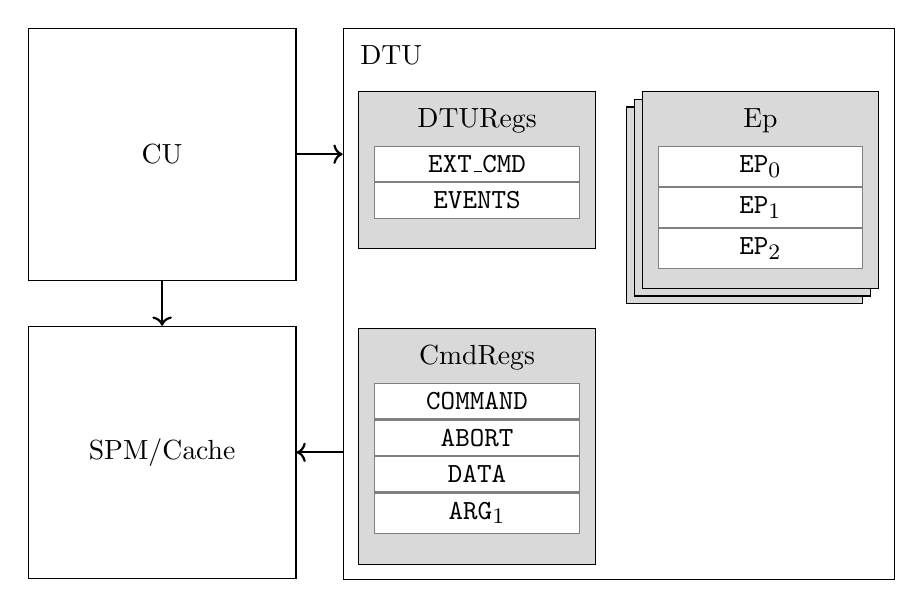
\begin{tikzpicture}[
      dtureg/.style={draw=gray,fill=white,minimum width=2.6cm},
      regtbl/.style={draw=black,fill=gray!30,minimum width=3cm}
    ]

    \node[draw=black,minimum width=7cm,minimum height=7cm,anchor=north west] (dtu) at(4,0) {};
    \node[draw=black,minimum width=3.4cm,minimum height=3.2cm,anchor=north west] (cu) at (0,0) {CU};
    \node[draw=black,minimum width=3.4cm,minimum height=3.2cm,anchor=south west] (mem) at (0,-7) {SPM/Cache};

    \node[below right=.1cm and .1cm of dtu.north west] {DTU};

    \node[
      regtbl,below right=.8cm and .2cm of dtu.north west,minimum height=2cm
    ] (dturegs) {};
    \node[below=.1cm of dturegs.north] {DTURegs};
    \node[dtureg,below=.7cm of dturegs.north] (dtureg0) {\texttt{EXT\_CMD}};
    \node[dtureg,below=0cm of dtureg0]        (dtureg1) {\texttt{EVENTS}};

    \node[
      regtbl,below=1cm of dturegs.south,minimum height=3cm
    ] (cmdregs) {};
    \node[below=.1cm of cmdregs.north] {CmdRegs};
    \node[dtureg,below=.7cm of cmdregs.north] (cmdreg0) {\texttt{COMMAND}};
    \node[dtureg,below=0cm of cmdreg0]        (cmdreg1) {\texttt{ABORT}};
    \node[dtureg,below=0cm of cmdreg1]        (cmdreg2) {\texttt{DATA}};
    \node[dtureg,below=0cm of cmdreg2]        (cmdreg3) {\texttt{ARG$_1$}};

    \node[
      regtbl,below left=1cm and .4cm of dtu.north east,minimum height=2.5cm
    ] {};
    \node[
      regtbl,below left=.9cm and .3cm of dtu.north east,minimum height=2.5cm
    ] {};
    \node[
      regtbl,below left=.8cm and .2cm of dtu.north east,minimum height=2.5cm
    ] (epregs) {};
    \node[below=.1cm of epregs.north] {Ep};
    \node[dtureg,below=.7cm of epregs.north] (epreg0) {\texttt{EP$_0$}};
    \node[dtureg,below=0cm of epreg0]        (epreg1) {\texttt{EP$_1$}};
    \node[dtureg,below=0cm of epreg1]        (epreg2) {\texttt{EP$_2$}};

    \path
      let \p1=(cu.east), \p2=(dtu.west) in
      [draw=black,thick,->] (cu.east) -- (\x2,\y1);
    \path[draw=black,thick,->] (cu) -- (mem);
    \path
      let \p1=(mem.east), \p2=(dtu.west) in
      [draw=black,thick,<-] (mem.east) -- (\x2,\y1);
  \end{tikzpicture}
  \caption{Overview of the DTU's registers and its connections to other components.}
  \label{fig:overview}
\end{figure}

As shown in \rref{fig:overview}, the compute unit~(CU) is connected to the data transfer unit~(DTU)
and can access the DTU's registers via memory mapped input/output (MMIO). Additionally, the CU is
connected to the local memory. The DTU is also connected to the local memory to, for example, access
messages. These components are not necessarily arranged in this way. For example, the DTU might
interpose itself between the CU and local memory.

\section{MMIO region}

The memory interface from CU to DTU is expected to be 64-bit wide. The MMIO region of the DTU is
defined as follows:

\vspace{2ex}
\noindent
\begin{tabular}{ p{3cm} | c | c | l }
  \textbf{Address} & \textbf{Register} & \textbf{Group} & \textbf{Description} \\
  \hline
  \texttt{0xF000\_0000} & \texttt{EXT\_CMD} & DtuRegs & Triggers external commands \\
  \hline
  \texttt{0xF000\_0008} & \texttt{EVENTS} & DtuRegs & Contains outstanding events \\
  \hline
  \texttt{0xF000\_0010} & \texttt{COMMAND} & CmdRegs & Triggers internal commands \\
  \hline
  \texttt{0xF000\_0018} & \texttt{ABORT} & CmdRegs & Aborts internal commands \\
  \hline
  \texttt{0xF000\_0020} & \texttt{DATA} & CmdRegs & Specifies the data for commands \\
  \hline
  \texttt{0xF000\_0028} & \texttt{ARG$_1$} & CmdRegs & Additional argument for commands \\
  \hline
  \texttt{0xF000\_0030} & \texttt{EP$_{00}$} & EpRegs & First register of EP$_0$ \\
  \texttt{0xF000\_0038} & \texttt{EP$_{01}$} & EpRegs & Second register of EP$_0$ \\
  \texttt{0xF000\_0040} & \texttt{EP$_{02}$} & EpRegs & Third register of EP$_0$ \\
  \hline
  \texttt{0xF000\_0048} & \texttt{EP$_{10}$} & EpRegs & First register of EP$_1$ \\
  \texttt{0xF000\_0050} & \texttt{EP$_{11}$} & EpRegs & Second register of EP$_1$ \\
  \texttt{0xF000\_0058} & \texttt{EP$_{12}$} & EpRegs & Third register of EP$_1$ \\
  \hline
  \multicolumn{4}{c}{\dots} \\
  \hline
  \texttt{0xF000\_0100} & \texttt{EP$_{n0}$} & EpRegs & First register of EP$_{n}$ \\
  \texttt{0xF000\_0108} & \texttt{EP$_{n1}$} & EpRegs & Second register of EP$_{n}$ \\
  \texttt{0xF000\_0110} & \texttt{EP$_{n2}$} & EpRegs & Third register of EP$_{n}$ \\
\end{tabular}

\section{Endpoints}

The DTU has a number of \emph{endpoints}~(EPs) to establish communication channels, which can be
configured to three different EP types: \emph{send EPs} and \emph{receive EPs} are used for message
passing, whereas \emph{memory EPs} are used for RDMA-like memory access. Each EP is represented by a
DTU register and can be configured (at runtime) to one of these EP types. Each EP consists of 192
bits, starting with 3 bits for the endpoint type (T) and 189 bits, whose meaning depends on the EP
type. T is either INVALID (0), SEND (1), RECEIVE (2), or MEMORY (3). The endpoints are defined as
follows:

\subsection{Memory EP}

\begin{scaletikzpicturetowidth}{.98\linewidth}
  \begin{tikzpicture}[
    baseline=8ex,scale=\tikzscale,
    reg/.style={fill=gray!20,draw=black},
    undef/.style={fill=gray!20,draw=black,pattern=north east lines, pattern color=black}
  ]
  \path[undef] (0,0) rectangle (33,3) node[midway] {};
  \path[reg] (33,0) rectangle (41,3) node[midway] {pe};
  \path[reg] (41,0) rectangle (45,3) node[midway] {rw};
  \path[undef] (45,0) rectangle (61,3) node[midway] {};
  \path[reg] (61,0) rectangle (64,3) node[midway] {T};
  \path[reg] (0,3) rectangle (64,6) node[midway] {base\_addr};
  \path[reg] (0,6) rectangle (64,9) node[midway] {size};

  \node[anchor=north west,xshift=-3pt] at (0,0)  {63};
  \node[anchor=north east,xshift=3pt]  at (64,0) {0};
  \end{tikzpicture}
\end{scaletikzpicturetowidth}

\begin{description}
  \item[size{[63:0]}:] the size of the region at the destination
  \item[base\_addr{[63:0]}:] the base address of the region at the destination
  \item[pe{[30:23]}:] the destination PE ID
  \item[rw{[22:19]}:] the permission bits (read = 1, write = 2)
\end{description}

\subsection{Send EP}

\begin{scaletikzpicturetowidth}{0.98\linewidth}
  \begin{tikzpicture}[
    baseline=8ex,scale=\tikzscale,
    reg/.style={fill=gray!20,draw=black},
    undef/.style={fill=gray!20,draw=black,pattern=north east lines, pattern color=black}
  ]
  \path[undef] (0,0) rectangle (18,3) node[midway] {};
  \path[reg] (18,0) rectangle (19,3) node[midway] {r};
  \path[reg] (19,0) rectangle (27,3) node[midway] {crd\_ep};
  \path[reg] (27,0) rectangle (33,3) node[midway] {msg\_sz};
  \path[reg] (33,0) rectangle (39,3) node[midway] {max\_crd};
  \path[reg] (39,0) rectangle (45,3) node[midway] {cur\_crd};
  \path[undef] (45,0) rectangle (61,3) node[midway] {};
  \path[reg] (61,0) rectangle (64,3) node[midway] {T};

  \path[undef] (0,3) rectangle (48,6) node[midway] {};
  \path[reg] (48,3) rectangle (56,6) node[midway] {pe};
  \path[reg] (56,3) rectangle (64,6) node[midway] {ep};
  \path[reg] (0,6) rectangle (64,9) node[midway] {label};

  \node[anchor=north west,xshift=-3pt] at (0,0)  {63};
  \node[anchor=north east,xshift=3pt]  at (64,0) {0};
  \end{tikzpicture}
\end{scaletikzpicturetowidth}

\begin{description}
  \item[label{[63:0]}:] the label the DTU puts into the header of each sent message
  \item[pe{[15:8]}:] the ID of the destination PE
  \item[ep{[7:0]}:] the ID of the receive EP
  \item[r{[45:45]}:] whether this is a reply EP
  \item[crd\_ep{[44:37]}:] for reply EPs: the send EP at sender-side to receive credits
  \item[max\_crd{[36:31]}:] the initially received (=max) credits (in messages)
  \item[cur\_crd{[30:25]}:] the currently owned credits (in messages)
  \item[max\_msg\_size{[24:19]}:] the maximum message size supported by the receiver
\end{description}

\subsection{Receive EP}

\begin{scaletikzpicturetowidth}{0.98\linewidth}
  \begin{tikzpicture}[
    baseline=8ex,scale=\tikzscale,
    reg/.style={fill=gray!20,draw=black},
    undef/.style={fill=gray!20,draw=black,pattern=north east lines, pattern color=black}
  ]
  \path[undef] (0,0) rectangle (7,3) node[midway] {};
  \path[reg] (7,0) rectangle (13,3) node[midway] {rpos};
  \path[reg] (13,0) rectangle (19,3) node[midway] {wpos};
  \path[reg] (19,0) rectangle (25,3) node[midway] {slot\_size};
  \path[reg] (25,0) rectangle (31,3) node[midway] {slots};
  \path[reg] (31,0) rectangle (39,3) node[midway] {rpl\_eps};
  \path[reg] (39,0) rectangle (45,3) node[midway] {msgs};
  \path[undef] (45,0) rectangle (61,3) node[midway] {};
  \path[reg] (61,0) rectangle (64,3) node[midway] {T};

  \path[reg] (0,3) rectangle (64,6) node[midway] {buffer};
  \path[reg] (0,6) rectangle (32,9) node[midway] {unread};
  \path[reg] (32,6) rectangle (64,9) node[midway] {occupied};

  \node[anchor=north west,xshift=-3pt] at (0,0)  {63};
  \node[anchor=north east,xshift=3pt]  at (64,0) {0};
  \end{tikzpicture}
\end{scaletikzpicturetowidth}

\begin{description}
  \item[unread{[63:32]}:] a bitmask with the unread (not yet fetched) messages in the buffer
  \item[occupied{[31:0]}:] a bitmask with the occupied slots in the buffer
  \item[buffer{[63:0]}:] the address of the receive buffer in local memory
  \item[rpos{[56:51]}:] the read position (for message fetches) within the receive buffer
  \item[wpos{[50:45]}:] the write position (for message receptions) within the receive buffer
  \item[slot\_size{[44:39]}:] the size of one slot as a power of 2
  \item[slots{[38:33]}:] the number of slots in the receive buffer as a power of 2
  \item[rpl\_eps{[32:25]}:] the offset of the reply EPs
  \item[msgs{[24:19]}:] the number of unread messages
\end{description}

\section{Commands}

The CU can use the DTU's endpoints via \emph{internal commands}. The command registers are used to
pass input arguments for a command to the DTU, start a command, and wait until the command is
finished. The following command registers are used:

\vspace{2ex}
\noindent
\begin{tabular}{ p{2cm} c }
  \texttt{COMMAND}: &
  \begin{scaletikzpicturetowidth}{0.8\linewidth}
    \begin{tikzpicture}[
      baseline=1ex,scale=\tikzscale,
      reg/.style={fill=gray!20,draw=black},
      undef/.style={fill=gray!20,draw=black,pattern=north east lines, pattern color=black}
    ]
    \path[reg] (0,0) rectangle (48,3) node[midway] {arg$_0$};
    \path[reg] (48,0) rectangle (52,3) node[midway] {err};
    \path[undef] (52,0) rectangle (53,3) node[midway] {};
    \path[reg] (53,0) rectangle (60,3) node[midway] {ep};
    \path[reg] (60,0) rectangle (64,3) node[midway] {op};

    \node[anchor=north west,xshift=-3pt] at (0,0)  {63};
    \node[anchor=north east,xshift=3pt]  at (64,0) {0};
    \end{tikzpicture}
  \end{scaletikzpicturetowidth}
  \\
  \\
  \texttt{DATA}: &
  \begin{scaletikzpicturetowidth}{0.8\linewidth}
    \begin{tikzpicture}[
      baseline=1ex,scale=\tikzscale,
      reg/.style={fill=gray!20,draw=black},
      undef/.style={fill=gray!20,draw=black,pattern=north east lines, pattern color=black}
    ]
    \path[reg] (0,0) rectangle (16,3) node[midway] {size};
    \path[reg] (16,0) rectangle (64,3) node[midway] {address};

    \node[anchor=north west,xshift=-3pt] at (0,0)  {63};
    \node[anchor=north east,xshift=3pt]  at (64,0) {0};
    \end{tikzpicture}
  \end{scaletikzpicturetowidth}
\end{tabular}
\vspace{2ex}

\begin{description}
  \item[arg0{[63:16]}:] the first argument for the command
  \item[err{[15:12]}:] the error code (0 = no error)
  \item[ep{[10:4]}:] the endpoint to use for the command
  \item[op{[3:0]}:] the command (opcode)
  \item[size{[63:48]}:] the size of the data in local memory
  \item[address{[47:0]}:] the address of the data in local memory
\end{description}

\noindent A write to the \texttt{COMMAND} register starts the command with opcode
\texttt{COMMAND.op}. The meaning of the three argument registers depends on the opcode.

\subsection{Pseudo Code Building Blocks}

The following sections use pseudo code to describe the behavior of the DTU commands, based on
several building blocks:

\begin{itemize}
  \item \texttt{read\_ep(id) -> EP}:\\
  read the DTU-internal EP register with the given id
  \item \texttt{write\_ep(id, EP)}:\\
  write \texttt{EP} to the DTU-internal EP register with given id
  \item \texttt{read\_mem(addr, size) -> data}:\\
  read \texttt{size} bytes from given address in local memory into \texttt{data}
  \item \texttt{write\_mem(data, addr, size)}:\\
  write \texttt{data} of \texttt{size} bytes to given address in local memory
  \item \texttt{read\_remote(pe, size, offset) -> data}:\\
  read \texttt{size} bytes from the given PE at given offset into \texttt{data}
  \item \texttt{write\_remote(data, pe, offset)}:\\
  write \texttt{data} to \texttt{offset} in the given PE
  \item \texttt{send\_msg(msg, pe, ep)}:\\
  send \texttt{msg} to endpoint \texttt{ep} at given PE
  \item \texttt{send\_ack()}:\\
  send ACK to the sending DTU
  \item \texttt{wait\_for\_ack()}:\\
  wait for the ACK the receiving DTU sends upon successfully storing the message into the receive
  buffer or an error occurred
  \item \texttt{find\_slot(mask, pos, slots, val) -> idx}:\\
  searches for a bit with value \texttt{val} in the given mask from bit 0 to bit $(1 << slots) - 1$,
  starting at \texttt{pos}. The function returns the position of the bit or $-1$ if none was found.
  \item \texttt{exit(error)}:\\
  stop the execution of the command, set \texttt{COMMAND.op} to 0 and \texttt{COMMAND.err} to given error
\end{itemize}

\subsection{Memory Access}

Memory access is performed with a memory EP based on the commands \texttt{READ} and \texttt{WRITE}. The commands behave as follows:

\subsubsection{\texttt{READ}}

\begin{algorithm}[H]
    $ep \gets$ read\_ep(COMMAND.ep)\;
    \uIf{ep.T != MEMORY}{exit(INV\_EP)}
    \uIf{ep.rw \& READ == 0}{exit(NO\_PERM)}
    \uIf{ep.base\_addr + COMMAND.arg$_0$ > ep.size}{exit(INV\_ARGS)}
    \BlankLine
    $data \gets read\_remote(ep.PE, DATA.size, ep.base\_addr + COMMAND.arg_0)$\;
    $write\_mem(data, DATA.address, DATA.size)$\;
    \BlankLine
    $COMMAND \gets 0$\;
    \caption{The DTU's \texttt{READ} command.}
\end{algorithm}

\subsubsection{\texttt{WRITE}}

\begin{algorithm}[H]
    $ep \gets$ read\_ep(COMMAND.ep)\;
    \uIf{ep.T != MEMORY}{exit(INV\_EP)}
    \uIf{ep.rw \& WRITE == 0}{exit(NO\_PERM)}
    \uIf{ep.base\_addr + COMMAND.arg$_0$ > ep.size}{exit(INV\_ARGS)}
    \BlankLine
    $data \gets read\_mem(DATA.address, DATA.size)$\;
    $write\_remote(data, ep.PE, ep.base\_addr + COMMAND.arg_0)$\;
    \BlankLine
    $COMMAND \gets 0$\;
    \caption{The DTU's \texttt{WRITE} command.}
\end{algorithm}

\subsection{Message Passing}

Message passing is performed between a send EP and a receive EP. Each send EP is connected to
exactly one receive EP, whereas each receive EP can receive from multiple send EPs. The send EP
supports the command \texttt{SEND}, whereas the receive EP supports \texttt{REPLY}, \texttt{FETCH},
and \texttt{ACK\_MSG}.

Each message consists of a header and a payload. The header is built by the DTU and the payload is
given by the application. The header is defined as:

\vspace{2ex}
\noindent
\begin{tabular}{ p{2cm} c }
  Header: &
  \begin{scaletikzpicturetowidth}{0.8\linewidth}
    \begin{tikzpicture}[
      baseline=8ex,scale=\tikzscale,
      reg/.style={fill=gray!20,draw=black},
      undef/.style={fill=gray!20,draw=black,pattern=north east lines, pattern color=black}
    ]
    \path[reg] (0,0) rectangle (16,3) node[midway] {reply\_size};
    \path[reg] (16,0) rectangle (32,3) node[midway] {length};
    \path[reg] (32,0) rectangle (40,3) node[midway] {rep};
    \path[reg] (40,0) rectangle (48,3) node[midway] {sep};
    \path[reg] (48,0) rectangle (56,3) node[midway] {spe};
    \path[reg] (56,0) rectangle (64,3) node[midway] {flags};
    \path[reg] (0,3) rectangle (64,6) node[midway] {reply\_label};
    \path[reg] (0,6) rectangle (64,9) node[midway] {label};

    \node[anchor=north west,xshift=-3pt] at (0,0)  {63};
    \node[anchor=north east,xshift=3pt]  at (64,0) {0};
    \end{tikzpicture}
  \end{scaletikzpicturetowidth}
\end{tabular}
\vspace{2ex}

\begin{description}
  \item[label{[63:0]}:] the label of the sender
  \item[reply\_label{[63:0]}:] the label the receiver should use for the reply
  \item[reply\_size{[63:48]}:] the size of the reply message as a power of 2
  \item[length{[47:32]}:] the payload size in bytes
  \item[rep{[31:24]}:] the receive endpoint ID for the reply at the sender side
  \item[sep{[23:16]}:] the sender endpoint ID
  \item[spe{[15:8]}:] the sender PE ID
  \item[flags{[7:0]}:] contains the following flags:
  \begin{itemize}
    \item \texttt{REPLY} (1): the message is a reply
    \item \texttt{GRANT\_CREDITS} (2): the receiver of the message should receive credits
    \item \texttt{REPLY\_ENABLED} (4): the receiver of the message may reply to the message
  \end{itemize}
\end{description}

\noindent The commands and the message reception behave as follows:

\subsubsection{\texttt{SEND}}

\begin{algorithm}[H]
    $ep \gets$ read\_ep(COMMAND.ep)\;
    \uIf{ep.T != SEND}{exit(INV\_EP)}
    \uIf{ep.cur\_crd != UNLIMITED}{
      \uIf{ep.cur\_crd == 0}{exit(NO\_CREDITS)}
      ep.cur\_crd -= 1\;
      $write\_ep(COMMAND.ep, ep)$\;
    }
    \BlankLine
    $rep \gets read\_ep(COMMAND.arg_0$)\;
    $header \gets$ \{ flags $\gets$ REPLY\_ENABLED\;
    $\quad\quad\quad\quad\quad label \gets ep.label$\;
    $\quad\quad\quad\quad\quad length \gets DATA.size$\;
    $\quad\quad\quad\quad\quad reply\_size \gets rep.slot\_size$\;
    $\quad\quad\quad\quad\quad reply\_label \gets ARG_1$\;
    $\quad\quad\quad\quad\quad spe \gets ownPE$\;
    $\quad\quad\quad\quad\quad sep \gets COMMAND.ep$\;
    $\quad\quad\quad\quad\quad rep \gets COMMAND.arg_0$ \}\;
    $payload \gets read\_mem(DATA.address, DATA.size)$\;
    $send\_msg(header\ |\ payload, ep.pe, ep.ep)$\;
    $wait\_for\_ack()$\;
    \BlankLine
    $COMMAND \gets 0$\;
    \caption{The DTU's \texttt{SEND} command.}
\end{algorithm}

\subsubsection{\texttt{RECEIVE}}

\begin{algorithm}[H]
    $ep \gets$ read\_ep(rep)\;
    \uIf{ep.T != RECEIVE}{exit(send\_ack() and drop message)}
    \BlankLine
    $idx \gets$ find\_slot(ep.occupied, ep.wpos, ep.slots, 0)\;
    \uIf{idx == -1}{exit(send\_ack() and drop message)}
    $ep.occupied.set\_bit(idx)$\;
    $ep.wpos \gets idx + 1$\;
    \BlankLine
    $dest \gets ep.buffer + (idx << ep.msg\_size)$\;
    $write\_mem(header\ |\ payload, dest, sizeof(header) + header.length)$\;
    ep.msgs += 1\;
    $ep.unread.set\_bit(idx)$\;
    $write\_ep(rep, ep)$\;
    \BlankLine
    \uIf{(header.flags \& REPLY) == 0}{
      $sep \gets$ \{ T \gets SEND$\;
      $\quad\quad\quad\ \  r \gets 1$ \}\;
      $\quad\quad\quad\ \  pe $\gets$ header.spe\;
      $\quad\quad\quad\ \  ep \gets header.rep$\;
      $\quad\quad\quad\ \  label \gets header.reply\_label$\;
      $\quad\quad\quad\ \  max\_msg\_size \gets header.reply\_size$\;
      $\quad\quad\quad\ \  max\_crd \gets 1$\;
      $\quad\quad\quad\ \  cur\_crd \gets 1$\;
      $\quad\quad\quad\ \  crd\_ep \gets header.sep$\;
      $write\_ep(ep.rpl\_eps + idx, sep)$\;
    }
    \BlankLine
    \uIf{header.flags \& GRANT\_CREDITS}{
      $sep \gets read\_ep(header.rep)$\;
      sep.cur\_crd += 1\;
      $write\_ep(header.rep, sep)$\;
    }
    $send\_ack()$\;
    \caption{If `header | payload' is received via EP `rep'.}
\end{algorithm}

\subsubsection{\texttt{REPLY}}

\begin{algorithm}[H]
    $ep \gets$ read\_ep(COMMAND.ep)\;
    \uIf{ep.T != RECEIVE or ep.rpl\_eps == 0xFF}{exit(INV\_EP)}
    \BlankLine
    $idx \gets (COMMAND.arg_0 - ep.buffer) >> ep.msg\_size$\;
    $sep = read\_ep(ep.rpl\_eps + idx)$\;
    \uIf{sep.T != SEND or sep.r == 0}{exit(INV\_ARGS)}
    \uIf{sep.cur\_crd == 0}{exit(NO\_CREDITS)}
    \BlankLine
    sep.cur\_crd -= 1\;
    $write\_ep(ep.rpl\_eps + idx, sep)$\;
    \BlankLine
    $header \gets$ \{ flags $\gets$ REPLY | GRANT\_CREDITS\;
    $\quad\quad\quad\quad\quad label \gets sep.label$\;
    $\quad\quad\quad\quad\quad length \gets DATA.size$\;
    $\quad\quad\quad\quad\quad reply\_size \gets 0$\;
    $\quad\quad\quad\quad\quad reply\_label \gets 0$\;
    $\quad\quad\quad\quad\quad spe \gets ownPE$\;
    $\quad\quad\quad\quad\quad sep \gets COMMAND.ep$\;
    $\quad\quad\quad\quad\quad rep \gets sep.crd\_ep$ \}\;
    $payload \gets read\_mem(DATA.address, DATA.size)$\;
    $send\_msg(header\ |\ payload, sep.pe, sep.ep)$\;
    $wait\_for\_ack()$\;
    \BlankLine
    $COMMAND \gets 0$\;
    \caption{The DTU's \texttt{REPLY} command.}
\end{algorithm}

\subsubsection{\texttt{FETCH}}

\begin{algorithm}[H]
    $ep \gets$ read\_ep(COMMAND.ep)\;
    \uIf{ep.T != RECEIVE}{exit(INV\_EP)}
    \uIf{ep.msgs == 0}{
      OFFSET $\gets$ 0\;
      exit(0)\;
    }
    \BlankLine
    $idx \gets$ find\_slot(ep.unread, ep.rpos, ep.slots, 1)\;
    $ep.unread.clear\_bit(idx)$\;
    ep.msgs -= 1\;
    $ep.rpos \gets idx + 1$\;
    $write\_ep(COMMAND.ep, ep)$\;
    \BlankLine
    $OFFSET \gets ep.buffer + (idx << ep.msg\_size)$\;
    $COMMAND \gets 0$\;
    \caption{The DTU's \texttt{FETCH} command.}
\end{algorithm}

\subsubsection{\texttt{ACK\_MSG}}

\begin{algorithm}[H]
    $ep \gets$ read\_ep(COMMAND.ep)\;
    \uIf{ep.T != RECEIVE}{exit(INV\_EP)}
    \BlankLine
    $idx \gets (COMMAND.arg_0 - ep.buffer) >> ep.msg\_size$\;
    $ep.occupied.clear\_bit(idx)$\;
    \uIf{ep.unread.bit\_set(idx)}{
      $ep.unread.clear\_bit(idx)$\;
      ep.msgs -= 1\;
    }
    $write\_ep(COMMAND.ep, ep)$\;
    \BlankLine
    \uIf{ep.rpl\_eps != 0xFF}{
      $sep \gets \{~T \gets INVALID~\}$\;
      $write\_ep(ep.rpl\_eps + idx, sep)$\;
    }
    \BlankLine
    $COMMAND \gets 0$\;
    \caption{The DTU's \texttt{ACK\_MSG} command.}
\end{algorithm}

\end{document}
